\documentclass[a4paper]{article}

\usepackage[utf8]{inputenc}
\usepackage[T1]{fontenc}
\usepackage{textcomp}
\usepackage{listings}
\usepackage{stmaryrd}
\usepackage{lmodern}
\usepackage{amsfonts}
\usepackage{titling}
\usepackage{lipsum}
\usepackage[left=1in, right=1in, bottom=1in, top=1in]{geometry}
\usepackage{amsthm}
\usepackage{tcolorbox}
\usepackage{varwidth}
\usepackage{hyperref}
\usepackage{xcolor}
\usepackage{graphicx}
\usepackage{makeidx}
\usepackage{tikz}
\usepackage{cases}
\usepackage{apacite}
\usepackage{tkz-berge}
\usepackage{url}
\usepackage{tgtermes}
\usepackage{sectsty}
\usepackage{subcaption}
\usepackage{setspace}
\usepackage{float}
\usepackage{amsmath, amssymb}


% figure support
\usepackage{import}
\usepackage{xifthen}
\pdfminorversion=7
\usepackage{pdfpages}
\usepackage{transparent}
\usepackage{color}
\newcommand{\incfig}[2][1]{%
    \def\svgwidth{#1\columnwidth}
    \import{./figures/}{#2.pdf_tex}
}

%mathstyling
\theoremstyle{plain}
\newtheorem{thm}{Theorem}[section]
\newtheorem{lem}[thm]{Lemma}
\newtheorem{prop}[thm]{Proposition}
\newtheorem*{cor}{Corollary}

\theoremstyle{definition}
\newtheorem{defn}{Definition}[section]
\newtheorem{conj}{Conjecture}[section]
\newtheorem{exmp}{Example}[section]
\newtheorem{axiom}{Axiom}
\theoremstyle{remark}
\newtheorem*{rem}{Remark}
\newtheorem*{note}{Note}

\definecolor{darkgreen}{rgb}{0.0, 0.5, 0.0}

\pdfsuppresswarningpagegroup=1
\lstset{
tabsize = 4, %% set tab space width
showstringspaces = false, %% prevent space marking in strings, string is defined as the text that is generally printed directly to the console
numbers = left, %% display line numbers on the left
commentstyle = \color{darkgreen}, %% set comment color
keywordstyle = \color{blue}, %% set keyword color
stringstyle = \color{red}, %% set string color
rulecolor = \color{black}, %% set frame color to avoid being affected by text color
basicstyle = \small \ttfamily , %% set listing font and size
breaklines = true, %% enable line breaking
numberstyle = \tiny,
  frame=none,
  xleftmargin=2pt,
  stepnumber=1,
  belowcaptionskip=\bigskipamount,
  captionpos=b,
  escapeinside={*'}{'*},
  language=haskell,
  tabsize=2,
  emphstyle={\bf},
  showspaces=false,
  columns=flexible,
  showstringspaces=false,
  morecomment=[l]\%,
}
\begin{document}
	\begin{titlepage}
	\begin{center}
	\large
	University of Warwick \\
	Department of Computer Science \\
	\huge
	\vspace{50mm}
	\rule{\linewidth}{0.5pt} \\
	CS262 \\
	\vspace{5mm}
	\Large
	Logic and Verification
	\rule{\linewidth}{0.5pt}
	\vspace{5mm}
	\begin{figure}[H]
	\centering
	
\includegraphics[width=0.4\textwidth]{crest_black.eps}
	\end{figure}
	\vspace{37mm}
	Cem Yilmaz \\
	\today
	\end{center}
	\end{titlepage}
	\newpage
	\tableofcontents
	\newpage
	\section{Prolog}
	Prolog is programming in logic. A programming paradigm that is imperative/procedural, functional and objected-oriented. Its basic principles are recursion and induction.
\subsection{Arithmetic}
	Prolog supports basic arithmetic operators, i.e.,
	\begin{align}
		+,-,*,/
	\end{align}
	There is also basic support for functions such as
	\begin{align}
		\sin(x), \cos(x), \abs(x), sqrt(x), \max(X,Y)
	\end{align}
	There are also numerical operators such as
	\begin{align}
		=:=, =/=, >, <, >=, =<
	\end{align}
	The $is/2$ predicate which assigns numerical value of right hand side to left hand side, and lastly the unification operator
	\begin{align}
		=
	\end{align}
	bind free variables to make the match other members.
	\section{Propositional Formulas}
	\begin{tcolorbox}[colback=black!3!white,colframe=black!60!white,title=\begin{defn}Propositional formulas \label{Propositional formulas}\end{defn}]
	Propositional Formulas are exactly those that can be constructed by a finite number of applications of the following rules:
	\begin{enumerate}
		\item Propositional variables $p,q,r,\ldots$ and $\top$ and $\bot$ are atomic formulas
		\item If $X$ is a formula then so is $\neg X$ 
		\item if $X$ and $Y$ are formulas then so is $(X \circ Y)$, where $\circ$ is a binary connective (e.g., $\land, \neg, \to ,\ldots$ )
	\end{enumerate}
	\end{tcolorbox}
	\begin{tcolorbox}[colback=black!3!white,colframe=black!60!white,title=\begin{defn}Parse Tree \label{Parse Tree}\end{defn}]
	We can conductively construct a parse tree for any propositional formula:
	\begin{itemize}
		\item For any atomic formula $X$, the parse tree has a single node labeled $X$.
		\item The parse tree for $\neg X$ has a node labeled $\neg$ as the root, and the parse tree for $X$ as the unique subtree of the root.
		\item The parse tree for $(X \circ Y)$ has a node labeled $\circ$ as the root, and the parse trees for $X$ and $Y$ as its left and right subtree.
	\end{itemize}
	\end{tcolorbox}
	\begin{tcolorbox}[colback=black!3!white,colframe=black!60!white,title=\begin{exmp}Parse Tree \label{Parse Tree}\end{exmp}]
Consider the statement and draw it as a parse tree
\begin{align}
	((p \land \neg q) \to (r \lor (q \to \neg p )))
\end{align}
\begin{figure}[H]
    \centering
    \incfig{parsetree}
    \caption{Parse Tree for the above statement}
    \label{fig:parsetree}
\end{figure}
\end{tcolorbox}
\begin{tcolorbox}[colback=black!3!white,colframe=black!60!white,title=\begin{defn}Recursion and Degrees \label{Recursion and Degrees}\end{defn}]
Based on our inductive definition, we can define recursive functions on formulas. They are defined as
\begin{align}
	deg(A) &= 0 & \text{if $A$ is an atomic formula} \\
	deg(\neg X) &= 1 + deg(X) & \text{ if $X$ is a formula} \\
	deg(X \circ Y) &= deg(X) + deg(Y) + 1 & \text{if $X$ and $Y$ are formulas}
\end{align}
\end{tcolorbox}
\begin{tcolorbox}[colback=black!3!white,colframe=black!60!white,title=\begin{thm}Degree and Inner Nodes \label{Degree and Inner Nodes}\end{thm}]
	The degree of a formula equals the number of inner nodes of the parse tree
	\begin{proof}
		Consider the base case of atomic formula $A$, for which $deg(A) = 0$. Its corresponding parse tree would be a single node of $A$. It has no children therefore it is a leaf and is not an inner node. Indeed, the fact that it is note an inner node and $deg(A) = 0$ we obtain that they're equal. \\
	Consider the inductive step of two cases:
	\begin{enumerate}
		\item $\neg X$ 
		\item $(X \circ Y)$
	\end{enumerate}
		For the first case, we have that
		\begin{align}
			deg(\neg X) = 1 + deg(X)
		\end{align}
		The corresponding parse tree would result in a parent node of $\neg$ and a child node of $X$. Therefore, by definition, we create a new inner node that corresponds to $+1$. The child would represent the $deg(X)$ as required. \\
		For the second case, we have that
		\begin{align}
			deg(X \circ Y) = 1 + deg(X) + deg(Y)
		\end{align}
		The corresponding parse tree would result in a parent node of $\circ$ and two child nodes of $X$ and $Y$. Therefore, by definition, we create a new inner node which corresponds to the $+1$. The two children would correspond to the $deg(X)$ and $deg(Y)$ respectively.
	\end{proof}
\end{tcolorbox}
\begin{tcolorbox}[colback=black!3!white,colframe=black!60!white,title=\begin{defn}Valuation \label{Valuation}\end{defn}]
A valuation is a mapping $v$ from the set of propositional formulas to the set of truth values $\{T,F\}$ satisfying the following conditions:
\begin{align}
	v(\top) &= T; \; v(\bot) = F \\
	v(\neg X)  &= \neg v(X) \\
	v(X \circ Y) &= v(X) \circ v(Y)
\end{align}
To examine all interesting valuations for a given formula, it is enough to specify $v$ for each variable. The value of all subformulas can then be deduced bottom-up (in the parse tree)
\end{tcolorbox}
\begin{tcolorbox}[colback=black!3!white,colframe=black!60!white,title=\begin{defn}Tautology \label{Tautology}\end{defn}]
A formula that evaluates to $T$ under all valuations is called a tautology
\end{tcolorbox}
\begin{tcolorbox}[colback=black!3!white,colframe=black!60!white,title=\begin{defn}Contradiction \label{Contradiction}\end{defn}]
A formula that evaluates to $F$ under all valuations is called a contradiction
\end{tcolorbox}
\begin{tcolorbox}[colback=black!3!white,colframe=black!60!white,title=\begin{defn}Satisfiable \label{Satisfiable}\end{defn}]
A formula that evaluates to $T$ for some valuation is called satisfiable
\end{tcolorbox}
 \begin{tcolorbox}[colback=black!3!white,colframe=black!60!white,title=\begin{defn}Propositional Consequence \label{Propositional Consequence}\end{defn}]
 We say that a formula $X$ is a consequence of a set $S$ of formulas, denoted by $S\vDash X$, provided that $X$ maps to $T$ under every valuation that maps every member of $S$ to $T$. For example, $X$ is a tautology if and only if $\varnothing \vDash X$ 
 \end{tcolorbox}
 \begin{tcolorbox}[colback=black!3!white,colframe=black!60!white,title=\begin{exmp}Propositional Consequence \label{Propositional Consequence}\end{exmp}]
         Let the formula $A = (p \lor v) \land (\neg q \lor \neg r)$. Let the formula $U = \{p, \neg q\}$. Consider the question $U \vDash A$.
	 It follows that it is a logical consequence. We have two possibilities:
	 \begin{table}[H]
	 	\centering
	 	\caption{Possibilities}
	 	\label{tab:label}
	 	\begin{tabular}{|c|c|c|}
			\hline
			$p$ & $T$ & $T$ \\
			$q$ & $F$ & $F$ \\
			$r$ & $T$ & $F$ \\
			\hline
	 	\end{tabular}
	 \end{table}
`	 Therefore it is true. Other examples include 
\begin{align*}
	p \lor q \vDash q
\end{align*}
is not true as for $q = F$ and $P = T$ we get $T \vDash F$. Another example is
\begin{align*}
	\{p, p\to q\} \vDash q
\end{align*}
is also true as we only care when both $p$ and $p\to q$ are true. We find that $q$ is also true when these are true.
 \end{tcolorbox}
 \begin{tcolorbox}[colback=black!3!white,colframe=black!60!white,title=\begin{thm}Connection of consequence and implication \label{Connection of consequence and implication}\end{thm}]
 		\begin{align}
 			U \vDash A \text{ iff } \bigwedge_{i \in U} A_i \to  A
 		\end{align}
 Where $U = \{A_1,A_2,\ldots,A_i\}$
 \end{tcolorbox}
\begin{tcolorbox}[colback=black!3!white,colframe=black!60!white,title=\begin{defn}Logical Equivalence \label{Logical Equivalence}\end{defn}]
Formulas are truth functions: each valuation maps the formula to $T$ or $F$. Formulas representing the same truth function are called logically equivalent. For example,
\begin{align}
p\to q = \neg p \lor q
\end{align}
\end{tcolorbox}
\begin{tcolorbox}[colback=black!3!white,colframe=black!60!white,title=\begin{defn}Completeness \label{Completeness}\end{defn}]
A set of connectives is said to be complete if we can represent every truth function $\{T,F\}^{n}\to \{T,F\}$ using only these connectives. 
\end{tcolorbox}
\begin{tcolorbox}[colback=black!3!white,colframe=black!60!white,title=\begin{defn}Proof By Construction \label{Proof By Construction}\end{defn}]
To create a formula that is logically equivalent to any function $f$ on variables $x_1,\ldots x_n$ given by its truth table, we do the following:
\begin{enumerate}
	\item For every valuation which maps to $T$ construct the conjunction $L_1 \land \ldots \land L_n$ where $L_j$ is $x_j$ if $x_j$ is assigned $T$ under the valuation and $L_j$ is $\neg x_j$ if $x_j$ is assigned $F$ under the valuation
	\item Take the disjunction of all conjunctions from the previous step
	\item For the function that is everywhere $F$, by convention take $\bot$
\end{enumerate}
This shows that $\{ \neg\, \land, \lor\}$ is complete. The resulting formula is called the disjunctive normal form (DNF) of $f$.
\end{tcolorbox}
\begin{tcolorbox}[colback=black!3!white,colframe=black!60!white,title=\begin{exmp}DNF Example \label{DNF Example}\end{exmp}]
        Consider the table
	\begin{table}[H]
		\centering
		\caption{DNF Example}
		\label{tab:dnf}
		\begin{tabular}{ccc||c}
		$p$& $q$ & $r$ & $f$ \\
		\hline
		$T$ & $T$ & $T$ & $T$ \\
		$T$ & $T$ & $F$ & $T$ \\
		$T$ & $F$ & $T$ & $F$ \\
		$T$ & $F$ & $F$ & $F$ \\
		$F$ & $T$ & $T$ & $F$ \\
		$F$ & $T$ & $F$ & $F$ \\
		$F$ & $F$ & $T$ & $F$ \\
		$F$ & $F$ & $F$ & $T$ 
		\end{tabular}
	\end{table}
	We now consider only rows that have $f$ as $T$, that is, the first $2$ rows and the last row. We express it as
	\begin{align*}
		L_1 &= p \land q \land r \\
		L_2 &= p \land q \land \neg r \\
		L_8 &= \neg p \land \neg q \land \neg r
	\end{align*}
	We then take the disjunction of our $L$, that is
	\begin{align*}
		L_1 \lor L_2 \lor L_8
	\end{align*}
\end{tcolorbox}
\begin{tcolorbox}[colback=black!3!white,colframe=black!60!white,title=\begin{defn}Normal Forms \label{Normal Forms}\end{defn}]
A formula in disjunctive normal form (DNF) is a disjunction of conjunction of literals. \\
A formula in conjunctive norma form (CNF) is a conjunction of disjunctions of literals.
\end{tcolorbox}
\begin{tcolorbox}[colback=black!3!white,colframe=black!60!white,title=\begin{thm}Normal Form Presence \label{Normal Form Presence}\end{thm}]
	Every boolean function has a CNF and a DNF. Furthermore, we can write the generalised disjunction as
	\begin{align}
		[X_1,X_2,\ldots X_n] &:= X_1 \lor X_2 \lor \ldots \lor X_n \\
		\langle X_1,X_2,\ldots X_n \rangle &:= X_1 \land X_2 \land \ldots \land X_n
	\end{align}
\end{tcolorbox}
\begin{tcolorbox}[colback=black!3!white,colframe=black!60!white,title=\begin{defn}alpha and beta formulas \label{alpha and beta formulas}\end{defn}]
We group all propositional formulas of the forms $\left( X \circ Y \right) $ and $\neg\left( X \circ Y \right) $ where $\circ$ is a binary operator into two categories, those that act conjunctively, and those that act disjunctively:
\begin{table}[H]
	\centering
	\caption{alpha and beta formulas}
	\label{tab:label}
	\begin{tabular}{|c|cc||c|cc|}
		$\alpha$ & $\alpha_1$ & $\alpha_2$ & $\beta$ & $\beta_1$ & $\beta_2$ \\
		\hline
		$X \land Y$ & $X$ & $Y$ & $\neg\left( X \land Y \right) $ & $\neg X$ & $\neg Y$ \\
		$\neg (X \lor Y)$ & $\neg X$ & $\neg Y$ & $X \lor Y$ & $X$ & $Y$ \\
		$\neg \left( X \to Y \right) $ & $X$ & $\neg Y$ & $X \to Y$ & $\neg X$ & $\neg Y$ \\
		$\neg (X \leftarrow Y)$ & $\neg X$ & $Y$ & $X \leftarrow Y$ & $X$ & $\neg Y$ \\
		$\neg (X \uparrow Y)$ & $X$ & $Y$ & $X \uparrow Y$ & $\neg X$ & $\neg Y$ \\
		$X \downarrow Y$ & $\neg X$ & $\neg Y$ & $\neg (X \downarrow Y)$ & $X$ & $Y$ \\
		$X \not\to Y$ & $X$ & $\neg Y$ & $\neg (X \not\to Y)$ & $\neg X$ & $Y$ \\
		$X \not\leftarrow Y$ & $\neg X$ & $Y$ & $\neg (X \not\leftarrow Y)$ & $X$ & $\neg Y$
	\end{tabular}
\end{table}	
Note that $\alpha$ formulas are used during a conjunctive $\left( \land \right) $ and $\beta$ formulas are used during a disjunctive $\left( \lor \right) $. 
\end{tcolorbox}
\begin{tcolorbox}[colback=black!3!white,colframe=black!60!white,title=\begin{thm}Conjunctive Normal Form Algorithm \label{Conjunctive Normal Form Algorithm}\end{thm}]
	Given any propositional formula $X$, start with $\langle [X]\rangle$. Given the current expansion  $\langle D_1,\ldots,D_n \rangle$ select one of the disjunctions $D_i$ that is not a disjunction of literals. Select a non-literal $N$ from $D_i$. 
	\begin{itemize}
		\item If $N$ is a $\beta-$formula, then replace $N$ by the two formula sequence $\beta_1$ and $\beta_2$.
		\item If $N$ is an $\alpha-$formula, then replace the disjunction $D_i$ with two disjunctions, one in which $N$ is replaced by $\alpha_1$, and one in which $N$ is replaced by $\alpha_2$.
	\end{itemize}
\end{tcolorbox}
\begin{tcolorbox}[colback=black!3!white,colframe=black!60!white,title=\begin{exmp}CNF expansion algorithm \label{CNF exapnsion algorithm}\end{exmp}]
        Consider the statement
                \begin{align}
                \neg \left( p \land \neg \bot \right)  \lor \neg \left( \top \uparrow q \right) 
                \end{align}
	We now follow the algorithm. We have
	\begin{align}
		\langle[\neg \left( p \land \neg \bot \right)  \lor \neg \left( \top \uparrow q \right)]\rangle &= \\
&= \langle [ \neg \left( p \land \neg \bot \right) ),\neg \left( \top \uparrow q \right) ]\rangle \\
&= \langle[ \neg p, \bot , \neg\left( \top \uparrow q \right) \rangle] \\
&= \langle [ \neg p, \bot, \top],[\neg p, \bot, q ] \rangle
		\end{align}
		The algorithm stops here, however, this form could be greatly simplified.
\end{tcolorbox}
\begin{tcolorbox}[colback=black!3!white,colframe=black!60!white,title=\begin{thm}Terminal of Alorithm \label{Terminal of Alorithm}\end{thm}]
	The algorithm terminates, regardless of which choices are made during the algorithm. \\
	Consider a rooted tree. A branch is a sequence of nodes starting at the root, descending towards one of the children in each step (unless no children are present). We say that the tree is finitely branching if every node has only finitely many children. 
	\begin{tcolorbox}[colback=black!3!white,colframe=black!60!white,title=\begin{lem}Konig's Lemma \label{Konig's Lemma}\end{lem}]
	        A tree that is finitely branching but infinite must have an infinite branch
	\end{tcolorbox}
	\begin{proof}
		Define the rank of a propositional formula as follows: \\
		Recursion anchor: $r(p) = r(\neg p) = 0$ for variables $p$ ; $r( \top) = r(\bot)=0$ and $r(\neg \top) = r\left( \neg \bot \right) = 1$. The recursive step is as follows:
		\begin{align}
			r(\neg \neg Z) = r(Z) + 1 \\
			r(\alpha) = r(\alpha_1)+r(\alpha_2) + 1 \\
			r(\beta) = r(\beta_1) + r(\beta_2) + 1
		\end{align}
		For a generalised disjunction we have
		\begin{align}
			r([X_1,\ldots,X_n]) = \sum_{i=1}^{n} r(X_i)
	\end{align}
	We assign the current conjunction of disjunctions $\langle D_1,\ldots,D_n \rangle$ a sequence of $n$ balls, by placing one ball labelled $r(D_i)$ for each disjunction $D_i$ into a box. We argue that each step of the algorithm corresponds to removing one ball from the box, and replacing it either by two balls with a lower number ($\alpha-$expansion) or by one ball with a lower number (in all other cases).
	\end{proof}
\end{tcolorbox}
\begin{tcolorbox}[colback=black!3!white,colframe=black!60!white,title=\begin{thm}Disjunctive Normal Form Algorithm \label{Disjunctive Normal Form Algorithm}\end{thm}]
	Given any propositional formula $X$, start with $[\langle X\rangle]$. Given the current expansion  $[D_1,\ldots,D_n]$ select one of the disjunctions $D_i$ that is not a disjunction of literals. Select a non-literal $N$ from $D_i$. 
	\begin{itemize}
		\item If $N$ is a $\alpha-$formula, then replace $N$ by the two formula sequence $\alpha_1$ and $\alpha_2$.
		\item If $N$ is an $\beta-$formula, then replace the disjunction $D_i$ with two disjunctions, one in which $N$ is replaced by $\beta_1$, and one in which $N$ is replaced by $\beta_2$.
	\end{itemize}
	We will omit the example as it is similar to the CNF.
\end{tcolorbox}
\section{Proof Systems}
\begin{tcolorbox}[colback=black!3!white,colframe=black!60!white,title=\begin{defn}Semantic Tableau \label{Semantic Tableau}\end{defn}]
The proof system takes the form of a tree, with nodes labelled by propositional formulas. We think of each branch as a conjunction of the formulas on that branch and think of the tree as the disjunction of all of its branches, in other words, a DNF. The expansion is as follows:
\begin{itemize}
	\item If $N = \neg \top$, then extend the branch by a node labelled $\bot$ at its end
	\item If $N = \neg \top$, then extend the branch by a node labelled $\top$ at its end
	\item If $N = \neg \neg Z$, then extend the branch by a node labelled $Z$ at its end
	\item If $N$ is an $\alpha-$formula, then extend the branch by two nodes labelled $\alpha_1$,$\alpha_2$ ($\alpha-$expansion) at its end.
	\item If $N$ is a $\beta-$formula, then add a left and right child to the final node of the branch, and label one of them $\beta_1$ and the other one $\beta_2$ ($\beta-$expansion)
\end{itemize}
A branch of tableau is closed if both $X$ and $\neg X$ occur on the branch for some formula $X$. A branch can also be closed if $\bot$ appears. A tableau is closed if every branch is also closed. If you want to prove that $X$ is a tautology, you want to prove that there is a closed tableau for $\neg X$. We write
\begin{align}
	\vdash_t X
\end{align}
if $X$ has a tableau proof. Lastly, a tableau is strict, if no formula has had an expansion rule applied to it twice on the same branch.
\end{tcolorbox}
\begin{tcolorbox}[colback=black!3!white,colframe=black!60!white,title=\begin{exmp}Semantic Tableau Example \label{Semantic Tableau Example}\end{exmp}]
        Consider
                \begin{align}
                \neg (( p \to (q \to r)) \to ((p \lor s) \to ((q\to r) \lor s)))
                \end{align}
		We initially have $\alpha$ rule where
		\begin{align}
			\alpha_1 &= p \to \left( q \to r \right) \\
			\alpha_2 &= \neg (( p \lor s) \to (( q\to r) \lor s ))
		\end{align}
		We now find that there is a $\beta$ rule in $\alpha_1$.
		\begin{align}
			\beta_1 &= \neg p \\
			\beta_2 & = q \to  r
		\end{align}
		Followed by another $\beta$ rule on $\beta_2$ :
		\begin{align}
			\beta_3 &= \neg q \\
			\beta_4 &= r
		\end{align}
		We now require to expand $\alpha_2$. However, we have lots of branches. Specifically, we have branches $\beta_1, \beta_3, \beta_4$. We will blindly decide to do the $\alpha_2$ expansion on $\beta_1$ branch.
		\begin{align}
			\alpha_1 &= p \lor s\\
			\alpha_2 &= \neg ((q \to r ) \lor s) 
		\end{align}
		The rest of the example is left as exercise.
\end{tcolorbox}
\begin{tcolorbox}[colback=black!3!white,colframe=black!60!white,title=\begin{thm}Soundness and Completeness \label{Soundness and Completeness}\end{thm}]
	The tableau system is sound, i.e., if $X$ has a tableau proof, then $X$ is a tautology. Furthermore, the tableau proof system is complete, i.e., if $X$ is a tautology, then the strict tableau system will terminate with a proof for it. Equivalent,
		\begin{align}
		\vdash_t X \text{ iff } \vDash X
		\end{align}
		First theorem follows from correctness proof of our DNF expansion algorithm given before. 
\end{tcolorbox}
\begin{tcolorbox}[colback=black!3!white,colframe=black!60!white,title=\begin{defn}Resolution Proof \label{Resolution Proof}\end{defn}]
If the semantic tableau proof is the one that mirrors a DNF, then the resolution proof mirrors a conjunctive normal form. In particular, we have the following rules
\begin{itemize}
	\item If $N = \neg \top$, then append a new disjunction where $N$ is replaced by $\bot$ 
	\item If $N = \neg \bot$, then append a new disjunction where $N$ is replaced by $\top$ 
	\item If $N = \neg \neg Z$, then append a new disjunction where $N$ is replaced by $Z$
	\item If $N$ is an $\alpha$ formula, then append two new disjunctions, one in which $N$ is replaced by $\alpha_1$, and one in which it is replaced by $\alpha_2$
	\item If $N$ is a $\beta$ formula, then append a new disjunction where $N$ is replaced by $\beta_1, \beta_2$
\end{itemize}
A sequence of resolution expansion applications is strict, if every disjunction has at most one resolution expansion rule applied to it. We now need a resolution rule stated as follows:\\
Suppose $D_1$ and $D_2$ are two disjunctions, with $X$ occurring in $D_1$ and $\neg X$ in $D_2$. Let $D$ be the result of the following:
\begin{itemize}
	\item Delete all occurrences of $X$ from $D_1$ 
	\item Delete all occurrences of $\neg X$ from $D_2$ 
	\item Combine the resulting disjunctions
\end{itemize}
There is a special case that contains $\bot$. In such case, delete $\bot$ and call the resulting disjunction the trivial resolvent. I.e.,
\begin{align}
	\langle [X,Y],[\neg X, Z] \rangle = \langle[X,Y],[\neg X, Z], [Y, Z] \rangle
\end{align}
A resolution expansion is closed if it contains the empty clause $[]$. A resolution proof for $X$ is a closed resolution expansion for $\neg X$. We write
\begin{align}
	\vdash_r X
\end{align}
If $X$ has a resolution proof.
\end{tcolorbox}
\begin{tcolorbox}[colback=black!3!white,colframe=black!60!white,title=\begin{exmp}Resolution Proof  Example \label{Resolution Proof  Example}\end{exmp}]
\begin{figure}[H]
	\centering
	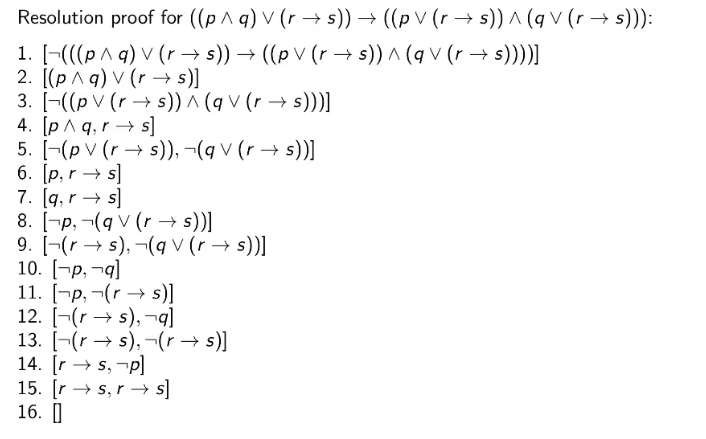
\includegraphics[width=0.8\textwidth]{one.png}
	\caption{Resolution Proof Example}
	\label{fig:one-png}
\end{figure}
\end{tcolorbox}
\begin{tcolorbox}[colback=black!3!white,colframe=black!60!white,title=\begin{thm}Soundness and Completeness \label{Soundness and Completeness}\end{thm}]
	The resolution proof system is sound, i.e., if $X$ has a resolution proof, then $X$ is a tautology.\\ 
	The resolution proof system is also complete, i.e., if $X$ is a tautology, then the resolution system will terminate with a proof for it, even if all resolution rule applications are atomic or trivial, and come after resolution expansion steps. Equivalently
	\begin{align}
		\vdash_r X \text{ iff } \vDash X
	\end{align}
	Similarly, our first theorem is an implication from the correctness proof of our CNF expansion algorithm given before. The resolution rule produces a semantically equivalent formula.
\end{tcolorbox}
\begin{tcolorbox}[colback=black!3!white,colframe=black!60!white,title=\begin{defn}S-introduction rule \label{S-introduction rule}\end{defn}]
The $S$-introduction rule for tableau says that for any formula $Y \in S$ can be added to the end of any tableau branch. We write $\vdash_t X$ if there is a closed tableau for $\neg X$ allowing the $S$-introduction rule for tableau. \\

The $S$-introduction rule for resolution states that for any formula $Y \in S$, the line $[Y]$ can be added as a line to a resolution expansion. We write $S \vdash_r X$ if there is a closed resolution expansion for $\neg X$, allowing the $S$-introduction rule for resolution.
\end{tcolorbox}
\begin{tcolorbox}[colback=black!3!white,colframe=black!60!white,title=\begin{thm}Strong soundness and completeness \label{Strong soundness and completeness}\end{thm}]
	For any set $S$ of propositional formulas and any formula $X$, we have
	\begin{align}
		S \vDash X \iff S \vdash_t X \iff S \vdash_r X
	\end{align}
\end{tcolorbox}
\begin{tcolorbox}[colback=black!3!white,colframe=black!60!white,title=\begin{exmp}S introduction Example \label{S introduction Example}\end{exmp}]
        Prove $\{ p\to q, q\to r\} \vDash \neg (\negr \land p)$ via tableau and resolution.
	\begin{proof}
		We begin our proof with tableau first.
		\begin{align}
			\neg \neg (\neg r \land p) &\\
			p \to q & \text{(note that we can add the $S$ rules whenever we want)} \\
			q \to r &\\
			\neg r \land p & \\
			\neg r & \\
			 p & \\
		\end{align}
		We now create a new branch below $p$ by expanding $p\to q$ 
		\begin{align}
			\neg p, q & \text{Note that $p$ is now closed.}
		\end{align}]
		And finally we expand $q \to r$ under $q$ 
		\begin{align}
			\neg q, r
		\end{align}
		And both branches close since we have $q$ and $\neg r$ above them. We now proof using the resolution proof.
		\begin{align}
			[ \neg \neg (\neg r \land p)] \\
			[p \to q] \\
			[q \to r] \\
			[\neg r \land p] \\
			[\neg p , q] \label{one} \\
			[\neg q, r] \label{two} \\
			[\neg r ] \label{three} \\
			[p] \label{four}
		\end{align}
		Let us combine \ref{one} and \ref{four}. We obtain
		\begin{align}
			[q] \label{five}
		\end{align}
		Then we resolution \ref{two} and \ref{three}:
		\begin{align}
			[\neg q] \label{six}
		\end{align}
		With the final resolution of \ref{five} and \ref{six}
		\begin{align}
			[]
		\end{align}
	\end{proof}
\end{tcolorbox}
\begin{tcolorbox}[colback=black!3!white,colframe=black!60!white,title=\begin{defn}Natural Deduction \label{Natural Deduction}\end{defn}]
Natural deduction formalizes the kind of reasoning people do in informal arguments. Unlike tableau and resolution, natural deduction is not well-suited for computer automation. It is also not based on CNF or DNF. \\
Implication rule. If one can derive $Y$ from $X$ as an assumption, then one can discharge the assumption and conclude that $X\to Y$ holds unconditionally. I.e.,
\begin{tcolorbox}[minipage,colback=white,arc=0pt,outer arc=0pt]
\centering
\begin{align*}
	X\\
	\vdots\\
	Y
\end{align*}
\end{tcolorbox}
means $X \to Y$. Subordinate proofs/lemmas are contained in boxes. The first formula $X$ is an assumption.
\begin{itemize}
	\item Modus Ponens Rule: From $X$ and $X\to Y$, we can conclude $Y$.
	\item Modus Tollens Rule: From $\neg Y$ and $X \to Y$, you can conclude $\neg Y$.
	\item Constant Rule: $\bot$ we can conclude any formula $X$, a contradiction. Similarly, we can always add $\top$ as it is always true.
	\item Negation Rules: If you have $X$ and $\neg X$, you can conclude $\bot$. Furthermore, if you have $X$ and $\bot$ in the same box, you can conclude $\neg X$.
	\item $\alpha E$: if you have an $\alpha$ rule, you can conclude $\alpha_1$ and/or $\alpha_2$ as you wish.
	\item $\alpha I$ : if you have $\alpha_1$ and $\alpha_2$, you can conclude $\alpha$ 
	\item $\beta E$ : if you have $\neg \beta_1$ and $ \beta$, you can conclude $\beta_2$. This can also be interchanged with $\beta$ numbers.
	\item $\beta I$: If you have $\neg \beta_1$ and $\beta 2$ in the same box, you can conclude $\beta$ out of the box. This rule can be interchanged with $\beta$ numbers.
\end{itemize}
A formula is called active at some stage if it does not occur in a closed box. The $E$ and $I$ are $Elimination$ and $Introduction$ respectively. There are also a set of derived rules, as follows:
\begin{itemize}
	\item Double negation: If you have $\neg \neg X$, you can conclude $X$. Similarly, if you have $X$ you can conclude $\neg \neg X$
	\item Copy rule: If you have $X $, you can conclude $X$ later down.
\end{itemize}
A good strategy for this proof system is to think backwards. What rules could be applied in the last step, and based on that come up with assumptions that should be made to apply those rules. Furthermore, in proving $X$ you can assume $\neg X$ and produce $\bot$, then use negation rule. Lecture 14 has a good example.
\end{tcolorbox}
\begin{tcolorbox}[colback=black!3!white,colframe=black!60!white,title=\begin{defn}S Introduction \label{S Introduction}\end{defn}]
$S-$ introduction rule for natural deduction is that at any stage, any member of $S$ may be used as a line. We write
\begin{align}
S \vdash_d X
\end{align}
If there is a natural deduction derivation of $X$ from $S$.
\end{tcolorbox}
\begin{tcolorbox}[colback=black!3!white,colframe=black!60!white,title=\begin{thm}Soundness and Completeness \label{Soundness and Completeness}\end{thm}]
	We have
		\begin{align}
	S \vDash X \iff S \vdash_d X	
		\end{align}
\end{tcolorbox}
\begin{tcolorbox}[colback=black!3!white,colframe=black!60!white,title=\begin{exmp}Natural Deduction Example \label{Natural Deduction Example}\end{exmp}]
        Find the natural deduction proof of
                \begin{align}
                (p\to (q\to r))\to (q\to (p\to r))
                \end{align}
		To begin this proof, we must create an assumption
		\begin{tcolorbox}[minipage,colback=white,arc=0pt,outer arc=0pt]
		\centering
		\begin{align}
			p \to (q\to r)& \text{ ass.}
		\end{align}
		\begin{tcolorbox}[minipage,colback=white,arc=0pt,outer arc=0pt]
		\centering
		\begin{align}
			q & \text{ ass.}
		\end{align}
		\begin{tcolorbox}[minipage,colback=white,arc=0pt,outer arc=0pt]
		\centering
		\begin{align}
			p &\text{ ass.} \\
			q \to r & \text{modus pon.} \\
			r 
		\end{align}
		\end{tcolorbox}
		\begin{align}
			p\to r & \text{ impl.}
		\end{align}
		\end{tcolorbox}
		\begin{align}
			q\to (p\to r) & \text{ impl.}
		\end{align}
		\end{tcolorbox}
\end{tcolorbox}
\section{Boolean Satisfiability Problem}
\begin{tcolorbox}[colback=black!3!white,colframe=black!60!white,title=\begin{defn}Problem SAT \label{Problem SAT}\end{defn}]
Given a propositional formula in conjunctive normal form, is there a satisfying assignment for it?
\end{tcolorbox}
\begin{tcolorbox}[colback=black!3!white,colframe=black!60!white,title=\begin{defn}Literal \label{Literal}\end{defn}]
A literal is a variable or a negated variable
\end{tcolorbox}
\begin{tcolorbox}[colback=black!3!white,colframe=black!60!white,title=\begin{defn}CNF Formula \label{CNF Formula}\end{defn}]
A formula in conjunctive normal form
\end{tcolorbox}
\begin{tcolorbox}[colback=black!3!white,colframe=black!60!white,title=\begin{defn}k-CNF Formula \label{k-CNF Formula}\end{defn}]
every clause has at most $k$ literals.
\end{tcolorbox}
\begin{tcolorbox}[colback=black!3!white,colframe=black!60!white,title=\begin{defn}k-SAT Problem \label{k-SAT Problem}\end{defn}]
Input of SAT is $k$-CNF
\end{tcolorbox}
\begin{tcolorbox}[colback=black!3!white,colframe=black!60!white,title=\begin{thm}Computational Complexity \label{Computational Complexity}\end{thm}]
	We can solve the problem SAT in time $2^{n} \times L$ by computing the entire truth table, where $L$ is the total number of literals of the input formula, and $n$ is the number of variables. This problem is the mother of all NP-complete problems.
\end{tcolorbox}
\begin{tcolorbox}[colback=black!3!white,colframe=black!60!white,title=\begin{thm}Satisfiability Iff \label{Satisfiability Iff}\end{thm}]
	There is a polynomial time algorithm that, given an instance $\mathcal{F}$ of SAT, produces a  $3$-CNF $\mathcal{G(F)}$ such that $\mathcal{F}$ is satisfiable if and only if $\mathcal{G(F)}$ is satisfiable
	\begin{proof}
		Consider a clause containing two literals $X$ and $Y$. Replace $X \lor Y$ in the clause by a new variable $Z$ (so the clause gets shorter by one literal) and express $X \lor Y \equiv Z$ by a $3$-CNF $H(X,Y,Z): [\ldots]$
	\end{proof}
\end{tcolorbox}
\begin{tcolorbox}[colback=black!3!white,colframe=black!60!white,title=\begin{defn}Reduction \label{Reduction}\end{defn}]
Problem Colouring. Given a graph $G=(V,E)$ and integer $k$, can its vertices be coloured properly with $k$ colours?\\
A colouring of $G$ is proper if the end vertices of every edge receive distinct colours.
\end{tcolorbox}
\begin{tcolorbox}[colback=black!3!white,colframe=black!60!white,title=\begin{thm}Coloring to SAT \label{Coloring to SAT}\end{thm}]
	There is a polynomial time algorithm that gives an instance $(G,k)$ of COLOURING, produces a CNF formula $\mathcal{F}(G,k)$ such that $G$ has a proper colouring with $k$ colours if and only if $\mathcal{F}(G,k)$ is satisfiable. \\
	In other words, if we can solve SAT efficiently, we can solve COLOURING efficiently. If we can count the number of satisfying assignments of a CNF formula efficiently, then we can count proper $k$-colourings efficiently.
	\begin{proof}
		For each vertex $v$ and each colour $k$, introduces a variable
		\begin{align}
			x_{v,k} = 
			\begin{cases}
				1 & \text{ if vertex $v$ receives colour $k$}\\
				0 & \text{ else}
			\end{cases}
		\end{align}
		We add constraints that every vertex receives exactly one colour. We then add constrains that the end vertices of every edge receive two distinct colours. We have $|V| \cdot k$ variables and the size of the formula we have polynomial in $|V|$ and $|E|$.
	\end{proof}
\end{tcolorbox}
\begin{tcolorbox}[colback=black!3!white,colframe=black!60!white,title=\begin{defn}Resolution \label{Resolution}\end{defn}]
We will solve $2$-SAT in polynomial time. Recall the resolution proof method, we maintain a conjunction of disjunctions. Our first step is resolution expansion into a CNF and the second step is the resolution rule.  \\
The key is observation is that the resolution clause of size $2$ produces another clause of size $\le 2$. At most $1+2n+4 {n \choose 2} = 2n^2+1$ clauses ever occur in the process. If formula is satisfiable, then the empty clause $[]$ will occur, otherwise it is satisfiable. 
\end{tcolorbox}
\begin{tcolorbox}[colback=black!3!white,colframe=black!60!white,title=\begin{defn}Linear-time algorithm for 2 SAT \label{Linear-time algorithm for 2 SAT}\end{defn}]
Recall that 
\begin{align}
u \lor v \equiv \neg u \to v \equiv \neg v \to u
\end{align}
The idea is to capture this implication information of a $2$-CNF $\mathcal{F}$ in a directed graph $D = D (\mathcal{F})$ :
\begin{itemize}
	\item Vertex set $V(D) := V \cup \overline{V}$, i.e., all variables $V = V(\mathcal{F})$ and their negation
	\item Edge set $E(D) := \{(\neg u , v), (\neg v , u) | [ u \lor v] \in \mathcal{F} \} \cup  \{(\neg u , u) | [u] \in \mathcal{F}\}$
\end{itemize}
$2$-clause lead to two directed edges, whereas a unit clause leads to a single directed edge. The graph $D$ has $2n$ vertices, where $n := |V|$, and at most $2m$ edges, where $m := |\mathcal{F}|$
\end{tcolorbox}
\begin{tcolorbox}[colback=black!3!white,colframe=black!60!white,title=\begin{exmp}Linear-time algorithm for 2 SAT \label{Linear-time algorithm for 2 SAT}\end{exmp}]
       Consider
                \begin{align}
               \mathcal{F} = \langle [\neg x_1, x_2],[\neg x_2,x_3],[\neg x_3,x_4],[\neg x_4, x_1] , [\neg x_5, x_3],[x_5, x_1] \rangle
                \end{align}
		Using algorithm we create the edges for each clause:
		\begin{itemize}
			\item $[\neg x_1, x_2] = x_1 \to x_2, \neg x_2 \to \neg x_1$ 
			\item $[\neg x_2, x_3] = x_2 \to x_3, \neg x_3 \to \neg x_2$
			\item $[ \neg x_3, x_4] = x_3 \to x_4, \neg x_4 \to \neg x_3$
			\item $[\neg x_4, x_1] = x_4 \to x_1, \neg x_1 \to \neg x_4$
			\item $[\neg x_5, x_3] = x_5 \to x_3, \neg x_3 \to  \neg x_5$
			\item $[x_5,x_1] = \neg x_5 \to  x_1 , \neg x_1 \to  x_5$
		\end{itemize}
\end{tcolorbox}
\begin{tcolorbox}[colback=black!3!white,colframe=black!60!white,title=\begin{defn}Directed Path \label{Directed Path}\end{defn}]
Write
\begin{align}
x \leadsto y
\end{align}
If there is a directed path from $x$ to $y$ in the graph $D(\mathcal{F})$.
\end{tcolorbox}
\begin{tcolorbox}[colback=black!3!white,colframe=black!60!white,title=\begin{lem}Satisfiability for linear time \label{Satisfiability for linear time}\end{lem}]
        $\mathcal{F}$ is not satisfiable if and only if there is a variable $x \in V$ such that $x \leadsto \neg x \leadsto x$
\end{tcolorbox}
\begin{tcolorbox}[colback=black!3!white,colframe=black!60!white,title=\begin{defn}Strongly Connected \label{Strongly Connected}\end{defn}]
Two vertices $u$ and $v$ in a directed graph are strongly connected if $u \leadsto v$ and $v \leadsto u$. The strongly connected components are the maximal subsets of vertices with this property.
\begin{proof}
	Let $\mathcal{F}'$ denote the CNF obtained from $\mathcal{F}$ by exhaustively applying resolution rule. Consider the resolvent $[u,v]$ of $[x,u]$ and $[\neg x,v]$. This resolvent would add two new edges to the graph, namely $\neg u \to v$ and $\neg v \to  u$. But the edges $\neg u \to  x \to  v$ and $\neg v \to  \neg x \to  u$ were already present. So adding these edges does not alter the relation $\leadsto$.  Therefore, $\mathcal{F}$ is not satisfiable if and only if $[]$ appears in $\mathcal{F}'$ if and only if $[x], [\neg x]$ appears in $\mathcal{F}'$ for some variable $x \in V$ if and only if $x \to  \neg x \to x$ in $D(\mathcal{F}')$ if and only if  $x \leadsto \neg x \leadsto x$.
\end{proof}
\end{tcolorbox}
\begin{tcolorbox}[colback=black!3!white,colframe=black!60!white,title=\begin{defn}Applications to 3-SAT \label{Applications to 3-SAT}\end{defn}]
We want to use our polynomial-time algorithms for solving $2$-SAT for solving $3$-SAT more efficiently, i.e., less than $2^{n}$ steps ($n$ is the number of variables). We consider the subset $\mathcal{G}$ of the independent definition of maximal size i.e., no further clauses can be obtained without violating independence.
\end{tcolorbox}
\begin{tcolorbox}[colback=black!3!white,colframe=black!60!white,title=\begin{defn}Independency \label{Independency}\end{defn}]
Given a $3$-CNF $\mathcal{F}$ over $n$ variables. A subset $\mathcal{G}$ of clauses of $\mathcal{F}$ is called independent if no two clases share any variables.
\end{tcolorbox}
\begin{tcolorbox}[colback=black!3!white,colframe=black!60!white,title=\begin{lem}Maximal Set and 3-SAT \label{Maximal Set and 3-SAT}\end{lem}]
        Consider a maximal set $\mathcal{G}$ of independent $3$-clause in $\mathcal{F}$. Then we have
	\begin{itemize}
		\item $|\mathcal{G}| \le \frac{n}{3}$
		\item For any truth assignment $\alpha$ to the variables in $\mathcal{G}$, $\mathcal{F}^{[\alpha]}$ is a $2$-CNF. Here, $\mathcal{F}^{[\alpha]}$ is the formula obtained from $\mathcal{F}$ by setting all variables defined by $\alpha$ to $T$ or $F$ (remove clauses with $T$ literals and remove $F$ literals from clauses)
		\item The number of truth assignments satisfying $\mathcal{G}$ is $7^{|\mathcal{G}|}\le 7^{\frac{n}{3}}$
	\end{itemize}
\end{tcolorbox}
\begin{tcolorbox}[colback=black!3!white,colframe=black!60!white,title=\begin{defn}3-SAT Algorithm \label{3-SAT Algorithm}\end{defn}]
Go through all truth assignments $\alpha$ satisfying $\mathcal{G}$, and check satisfiability of the $2$-CNF $\mathcal{F}^{[\alpha]}$ in polynomial time (quadratic or linear)
\end{tcolorbox}
\begin{tcolorbox}[colback=black!3!white,colframe=black!60!white,title=\begin{thm}3-CNF Runtime \label{3-CNF Runtime}\end{thm}]
	Satisfiability of a $3$-CNF formula can be decided in time
		\begin{align}
		O(7^{\frac{n}{3}}\text{poly}(n)) = O(1.913^{n})
		\end{align}
\end{tcolorbox}
\begin{tcolorbox}[colback=black!3!white,colframe=black!60!white,title=\begin{defn}Horn Satisfiability \label{Horn Satisfiability}\end{defn}]
We sat that $2$-SAT is a special case of SAT that can be solved efficiently. We now consider another special case, where there is no restriction on the size of clauses, but on their structure.
\end{tcolorbox}
\begin{tcolorbox}[colback=black!3!white,colframe=black!60!white,title=\begin{defn}Horn Clause \label{Horn Clause}\end{defn}]
A horn clause is a clause in which there is at most one positive literal (non-negated value)
\end{tcolorbox}
\begin{tcolorbox}[colback=black!3!white,colframe=black!60!white,title=\begin{defn}Horn CNF \label{Horn CNF}\end{defn}]
A horn CNF is a CNF that only has Horn clauses
\end{tcolorbox}
\begin{tcolorbox}[colback=black!3!white,colframe=black!60!white,title=\begin{defn}Satisfiability of Horn CNF \label{Satisfiability of Horn CNF}\end{defn}]
If every clause has size $\ge 2$, then the formula can be satisfied by setting all variables to $F$. If the formula has a clause of size $1$, then we have to set the literal in this clause to $T$ to satisfy the formula. If the formula contains the empty clause $[]$, then the formula is not satisfiable. If $\mathcal{F}$ is a Horn CNF, then $\mathcal{F}^{[\alpha]}$ is also a Horn CNF for any assignment $\alpha$. These observations give the algorithm
\begin{lstlisting}[language = pseudo , caption={Horn CNF Linear Time} , frame = trBL , firstnumber = last , escapeinside={(*@}{@*)}]
Input: Horn CNF (*@$\mathcal{F}$@*)
Output: 'Yes' if (*@$\mathcal{F}$@*) is satisfiable, 'No' otherwise
while (*@$([] \not \in \mathcal{F})$@*) {
	If (*@$\mathcal{F} = \langle \rangle$@*) or every clause in (*@$\mathcal{F}$@*) has size (*@$ \ge 2$@*), return 'Yes'
	Pick a clause (*@$[u] \in \mathcal{F}}$@*) of size (*@$=1$@*)
	Remove all clauses containing (*@$u$@*) from (*@$\mathcal{F}$@*), and remove all literal (*@$ \eg u$@*) from all clauses containing it
}
return 'No'
\end{lstlisting}
\end{tcolorbox}
\begin{tcolorbox}[colback=black!3!white,colframe=black!60!white,title=\begin{defn}Naive Backtracking Algorithm \label{Naive Backtracking Algorithm}\end{defn}]
\begin{lstlisting}[language = psuedo , caption={Naive Backtracking Algorithm} , frame = trBL , firstnumber = last , escapeinside={(*@}{@*)}]
Input: CNF formula (*@$F$@*)
Output: Satisfying assignment if one exists, (*@$\bot$@*) otherwise
if (*@$F = \langle \rangle$@*) then
	return (*@$\varnothing$@*)	
else if (*@$[] \in \mathcal{F}$@*) then
	return (*@$\bot$@*)
else
	Let (*@$l$@*) be a literal in (*@$ \mathcal{F}	$@*) and set (*@$L :=$@*)Back(*@$(\mathcal{F} | l)$@*)
	if (*@$ L \neq \bot $@*) return (*@$L \cup \{ l \}$@*) else set (*@$L :=$@*)Back(*@$(\mathcal{F}| \neg l)$@*)
	if (*@$L \neq \bot $@*) return (*@$L \cup \{ \neg l \}$@*) else return (*@$\bot$@*)
\end{lstlisting}
$\mathcal{F} | l$ denotes the formula obtained by setting $l := T$, i.e., we remove all clauses containing $l$ and all occurrences of $\neg l$. In the computed assignment $L$, membership $l \in L$ means that literal $l$ is set to $T$.\\
However, we can improve this algorithm with two observations. Unit clauses $[l]$ force the assignment $l := T$; we call it unit clause propagation. Furthermore, pure literals, i.e., literals $l$ for which $\neg l$ does not appear in the current formula, can be set to $l := T$. In other words,
\begin{lstlisting}[language = pseudo , caption={UnitPure} , frame = trBL , firstnumber = last , escapeinside={(*@}{@*)}]
Input: CNF formula (*@$\mathcal{F}$@*)
Output: Partial assignment
(*@$L := \varnothing; \mathcal{F}' := \mathcal{F}$@*)
while (*@$\mathcal{F'}$@*) contains a unit clause (*@$[l]$@*) or a pure literal (*@$l$@*) do
	(*@$L := L \cup \{l \}$@*)
	(*@$ \mathcal{F}' := \mathcal{F}' | l$@*)
return L
\end{lstlisting}
\end{tcolorbox}
\begin{tcolorbox}[colback=black!3!white,colframe=black!60!white,title=\begin{defn}DPLL Algorithm \label{DPLL Algorithm}\end{defn}]
DPLL is the Davis-Putnam-Logemann-Loveland algorithm
\begin{lstlisting}[language = pseudo , caption={DPLL(G)} , frame = trBL , firstnumber = last , escapeinside={(*@}{@*)}]
Input: CNF formula (*@$\mathcal{G}$@*)
Output: Satisfying assignment if one exists, (*@$\bot$@*) otherwise
(*@$U := $@*)UnitPure(*@$(\mathcal{G})$@*)
(*@$\mathcal{F} := \mathcal{G} | U$@*)
If (*@$\athcal{F} = \langle \rangle$@*) then
	return (*@$\varnothing$@*)
else if (*@$[] \in \mathcal{F}$@*) then
	return (*@$\bot$@*)
else
	Let (*@$l$@*) be a literal in (*@$\mathcal{F}$@*) and set (*@$L:=$@*)DPLL(*@$(\mathcal{F} | l)$@*)
	if (*@$L \neq \bot$@*) return (*@$U \cup L \cup \{l\}$@*) else set (*@$L :=$@*)DPLL(*@$(\mathcal{F} | \neq l)$@*)
	if (*@$ L \neq \bot$@*) return (*@$U \cup L \cup \{ \neq l \}$@*) else return (*@$\bot$@*)
\end{lstlisting}
However, which literal $l$ to choose in the next recursion step and which branch $l$ or $\neg l$ first? \\
Static heuristics linear ordering of variables fixed before start, usually very fast to compute, and thus also use more expensive algorithms. Or we could try dynamic heuristics, where we determine ordering based on current formula $\mathcal{F}$, typically from number of occurrences of literals.
\end{tcolorbox}
\begin{tcolorbox}[colback=black!3!white,colframe=black!60!white,title=\begin{defn}DLIS \label{DLIS}\end{defn}]
Dynamic Largest Individual Sum is when we choose literal which occurs most frequently
\end{tcolorbox}
\begin{tcolorbox}[colback=black!3!white,colframe=black!60!white,title=\begin{defn}MOMS \label{MOMS}\end{defn}]
Maximum occurrence in clauses of minimum size, i.e., we choose literal which occurs most frequently in clauses of minimum size
\end{tcolorbox}
\begin{tcolorbox}[colback=black!3!white,colframe=black!60!white,title=\begin{defn}Implication Graph \label{Implication Graph}\end{defn}]
The implication graph is a directed graph associated with any particular stage of the algorithm
\begin{itemize}
	\item For each literal $l$ set to true, called a decision literal, the graph contains a node labelled $l$ 
	\item For any clause $C = [l_1,\ldots,l_k,l]$, where $\neg l_1, \ldots, \neg l_k$ are nodes, add a new node $l$ and edges from $\neg l_i \to l$ for all $i = 1,\ldots,k$. These edges correspond to the clause $C$.
\end{itemize}
\begin{figure}[H]
	\centering
	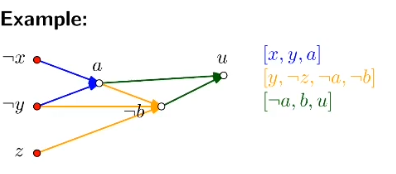
\includegraphics[width=0.6\textwidth]{two.png}
	\caption{Implication Graph Example}
	\label{fig:two-png}
\end{figure}
A conflict literal $l$ is one for which both $l$ and $\neg l$ appear as nodes in the graph. A conflict graph is a sub graph of the implication graph that contains exactly one conflict literal $l$, only nodes that have a path to $l$ or $\neg l$, and for every node only the incoming edges corresponding to one particular clause
\end{tcolorbox}
\begin{tcolorbox}[colback=black!3!white,colframe=black!60!white,title=\begin{defn}CDCL Algorithm \label{CDCL Algorithm}\end{defn}]
CDCL, the conflict-driven clause learning works as follows:
\begin{enumerate}
	\item Select a variable and assign $T$ or $F$ 
	\item Apply unit clause propagation
	\item Build the implication graph
	\item If there is any conflict
		\begin{enumerate}
			\item Derive a corresponding conflict clause and add it to the formula
			\item Non-chronologically backtrack ("back jump") to the decision level where the first-assigned variable involved in the conflict was assigned
		\end{enumerate}
	\item Continue from step $1$ until all variable values are assigned
\end{enumerate}
\begin{align}

\end{align}
\end{tcolorbox}
\section{First Order Logic}
\begin{tcolorbox}[colback=black!3!white,colframe=black!60!white,title=\begin{defn}First-Order Language \label{First-Order Language}\end{defn}]
A first-order language is determined by specifying:
\begin{itemize}
	\item A finite or countable set $\mathbf{R}$ of relation symbols, or predicate symbols. Each has some number of arguments
	\item A finite or countable set $\mathbf{F}$ of function symbols. Each has some number of arguments
	\item A finite or countable set $\mathbf{C}$ of constant symbols
\end{itemize}
We use $L(\mathbf{R},\mathbf{F}, \mathbf{C})$ for the first-order language determined by $\mathbf{R}$, $\mathbf{F}$, $\mathbf{C}$. Sometimes it is useful to think of constant symbols as function symbols with $0$ arguments.
\end{tcolorbox}
\begin{tcolorbox}[colback=black!3!white,colframe=black!60!white,title=\begin{defn}Model \label{Model}\end{defn}]
A model for the first order language $L(\mathbf{R},\mathbf{F},\mathbf{C})$ is a pair $\mathbf{M}=(\mathbf{D},\mathbf{I})$ where
\begin{itemize}
	\item $\mathbf{D}$ is a nonempty set, called the domain of $\mathbf{M}$.
	\item $\mathbf{I}$ is a mapping, called an interpretation that associates:
		\begin{itemize}
			\item To every constant symbol $c \in \mathbf{C}$, some member $c^{I} \in \mathbf{D}$ 
			\item To every function symbol $f \in \mathbf{F}$ with $n$ arguments, some $n$-ary function $f^{I}: \mathbf{D}^{n}\to \mathbf{D}$ 
			\item To every function symbol $R \in \mathbf{R}$ with $n$ arguments, some $n$-ary relation $R^{I}\subseteq \mathbf{D}^{n}$
		\end{itemize}
\end{itemize}
An assignment in a model $\mathbf{M} = (\mathbf{D},\mathbf{I})$ is a mapping $\mathbf{A}$ from the set of variables to the set $\mathbf{D}$. We write $x^{\mathbf{A}}$ for the image of $x$ under $\mathbf{A}$.
\end{tcolorbox}
\begin{tcolorbox}[colback=black!3!white,colframe=black!60!white,title=\begin{defn}Values of terms \label{Values of terms}\end{defn}]
Let $\mathbf{M} = (\mathbf{D},\mathbf{I})$ be a model for the language $L(\mathbf{R},\mathbf{F},\mathbf{C})$, and let $\mathbf{A}$ be an assignment in this model. To each term $t$ of the language, we associate a value $t^{\mathbf{I},\mathbf{A}}$ as follows:
\begin{itemize}
	\item For a constant symbol $c, c^{\mathbf{I},\mathbf{A}} = c^{\mathbf{I}}$ 
	\item For a variable $x$, $x^{\mathbf{I},\mathbf{A}} = x^{\mathnf{A}}$
	\item For a function symbol  $f$ with $n$ arguments, $(f(t_1,\ldots,t_n))^{\mathbf{I},\mathbf{A}} = f^{\mathbf{I}}(t_1^{\mathbf{I},\mathbf{A}},\ldots,t_n^{\mathbf{I},\mathbf{A}})$
\end{itemize}
\end{tcolorbox}
\begin{tcolorbox}[colback=black!3!white,colframe=black!60!white,title=\begin{defn}Example \label{Example}\end{defn}]
Suppose $L$ has a constant symbol $0$, a $1$-argument function symbol $s$, and a $2$-argument function symbol $+$. Consider the terms $t_1 := s(s(0)+s(x))$ and $t_2 := s(x+s(x+s(0)))$. \\
$\mathbf{D} = \{0,1,2,\ldots \}$, $0^{I}=0$, $s^{I}$ is the successor function, and $+^{I}$ is the addition operation. If $\mathbf{A}$ is an assignment such that $x^{\mathbf{A}} = 3$, then we have $t_1^{\mathbf{I},\mathbf{A}} = 6$ and $t_2^{\mathbf{I},\mathbf{A}} = 9$. More generally, $t_1^{\mathbf{I},\mathbf{A}} = x^{\mathbf{A}} +3$ and $t_2^{\mathbf{I},\mathbf{A}} = 2 x^{\mathbf{A}}+3$ \\
$\mathbf{D}$ is the set of all words over the alphabet $\{a,b \}$, $0 ^{I}= a$, $s^{\mathbf{I}}$ appends $a$ to the end of a word, and $+^{\mathbf{I}}$ is the concatenation. If $\mathbf{A}$ is an assignment such that $x^{\mathbf{A}} = aba$ , then $t_1^{\mathbf{I},\mathbf{A}} = aaabaaaa$ and $t_2^{\mathbf{I},\mathbf{A}}=abaabaaaaa$
\end{tcolorbox}
\begin{tcolorbox}[colback=black!3!white,colframe=black!60!white,title=\begin{defn}Truth of formulas \label{Truth of formulas}\end{defn}]
Let $\mathbf{M} = (\mathbf{D},\mathbf{I})$ be a model for the language $L$ and let $\mathbf{A}$ be an assignment to this model. To each $\phi$ of $L$, we associate a truth value $\phi^{\mathbf{I},\mathbf{A}}$ as follows:
\begin{itemize}
	\item $R(t_1,\ldots,t_n)^{\mathbf{I},\mathbf{A}} = T \iff (t_1^{\mathbf{I},\mathbf{A}},\ldots,t_n^{\mathbf{I},\mathbf{A}})\in R^{I}$
\end{itemize}

\end{tcolorbox}
\begin{tcolorbox}[colback=black!3!white,colframe=black!60!white,title=\begin{defn}Gamma and Delta Formulas \label{Gamma and}\end{defn}]
We extend the notation of $\alpha$ and $\beta$ formulas for our first order logic formulas. Namely, we have
\begin{table}[H]
	\centering
	\caption{Gamma and Delta}
	\label{tab:label}
	\begin{tabular}{cc|cc}
	$\gamma$ & $\gamma(t)$ & $\delta$ & $\delta(t)$ \\
	\hline
	$\forall x \phi$ & $\phi(\frac{x}{t})$ & $\exists \phi$ & $\phi(\frac{x}{t})$ \\
	$\neg \exists x \phi$ & $\neg \phi(\frac{x}{t})$ & $\neg \forall  x \phi$ & $\neg \phi ( \frac{x}{t})$
	\end{tabular}
\end{table}
	Here, $\phi(\frac{x}{t})$ denotes the formula obtained from $\phi$ by substituting the free occurrences of the variable $x$ by the term $t$.
\end{tcolorbox}
\begin{tcolorbox}[colback=black!3!white,colframe=black!60!white,title=\begin{exmp}Tableau Example \label{Tableau Example}\end{exmp}]
        Consider the statement
                \begin{align}
                \phi := \forall x(P(x) \lor Q(x)) \to  (\exists x P(x) \lor \forallx Q(x))
                \end{align}
		Consider
		\begin{align}
			\neg \phi &= \neg (\forall x(P(x) \lor Q(x)) \to  (\exists x P(x) \lor \forall xQ(x))) \\
			\forall x (P(x) \lor Q(x))  & \text{ $\alpha$ expansion}\\ 
			\neg (\exists x P(x) \lor \forall  x Q(x)) )& \text{ $ \alpha$ expansion} \\
			\neg \exists x P(x) & \text{ $\alpha$ expansion on second}\\
		\neg \forall x Q(x)	& \text{ $ \alpha$ expansion on second}	\\
		\neg Q(p) & \text{ $\delta$ with new parameter $p$} \\
		P(p)  \lor Q(p) & \text{ $\gamma$ with existing parameter $p$ on first equation}\\
		\neg P(p) & \text{ $\gamma$ with existing parameter $p$} 
		\end{align}
		We now apply $\beta$ expansion, creating two new branches on our $\lor$ statement.
		\begin{align}
			P(p) & Q(p)
		\end{align}
		Since we have $\neg Q(p)$ and $\neg P(p)$ above the  $\beta$ branch, we can close both branches. Our proof is finished.
\end{tcolorbox}
\begin{tcolorbox}[colback=black!3!white,colframe=black!60!white,title=\begin{exmp}Resolution \label{Resolution}\end{exmp}]
        Consider the statement
                \begin{align}
                [\neg(\phi := \forall x(P(x) \lor Q(x)) \to  (\exists x P(x) \lor \forallx Q(x)))]
                \end{align}
		We now notice $\alpha$ expansion
		\begin{align}
			[\forall x (P(x) \lor Q(x))]\\
			[\neg (\exists x P(x) \lor \forall x Q(x))] \\
			[ \neg \exists  x P(x) ] \\
			[\neg \forall x Q(x) ] \\
			[\neg Q (p)] \\
			[\neg P(p)] \\
			[P(p) \lor Q(p) ] \\
			[P(p), Q(p)]  \\
			[P(p)] \\
			[]
		\end{align}
\end{tcolorbox}
\begin{tcolorbox}[colback=black!3!white,colframe=black!60!white,title=\begin{defn}Natural Deduction \label{Natural Deduction}\end{defn}]
For natural deduction, we have two new rules for $\gamma E$:
\begin{table}[H]
	\centering
	\caption{Gamma Rule}
	\label{tab:label}
	\begin{tabular}{c|c}
		$\gamma$ & $\delta$ \\
		\hline
		$\gamma(t)$ & $\delta(p)$
	\end{tabular}
\end{table}
\end{tcolorbox}
\begin{tcolorbox}[colback=black!3!white,colframe=black!60!white,title=\begin{exmp}Natural Deduction Example \label{Natural Deduction Example}\end{exmp}]
        Consider the statement
                \begin{align}
			\phi := \forall x (P(x) \to  Q(x)) \to (\forall x P(x) \to \forall x Q(x))
                \end{align}
\begin{tcolorbox}[minipage,colback=white,arc=0pt,outer arc=0pt]
\centering
\begin{align*}
	\neg \phi \\
	\forall x (P(x) \to Q(x)) &\\
	\neg (\forall x P(x) \to  \forall x Q(x)) & \text{ $\alpha E$}\\
	\forall x P(x) &\\
	\neg \forall x Q(x) & \text{ $\alpha E$}\\
	\neg Q(p) & \text{ new variable $p$ from $\delta$} \\
	P(p) & \text{ $\gamma$ rule with $t=p$} \\
	P(p) \to  Q(p) & \text{ $\gamma$ rule with $t=p$}\\
	Q(p) & \text{ modus ponens}\\
	\bot
\end{align*}
\end{tcolorbox}
\end{tcolorbox}
\begin{tcolorbox}[colback=black!3!white,colframe=black!60!white,title=\begin{exmp}Example with multiple gamma and delta \label{Example with multiple gamma and delta}\end{exmp}]
        Consider
                \begin{align}
                F(x,y,z) := \exists x \forall y \forall z (P(y) \to Q(x)) \to ( P(x) \to Q(x))
                \end{align}
		We will prove this using tableau.
		\begin{align}
			\neg \exists x \forall y \forall z (P(y) \to Q(x)) \to ( P(x) \to Q(x)) & \\
			\neg \forall y \forall z F(p,y,z) & \text{ where $p$ is an existing parameter} \\
			\neg \forall z F(p,q,z) & \text{ where $q$ is a new parameter}\\ 
			\neg F ( p,q,r) & \text{ where $r$ is a new parameter} \\
			\neg \forall  y \forall z F(q,y,z) & \text{ $\gamma$ with now existing term $q$} \\
			\neg F(q,q',r') & \text{ where $q', r'$ are new parameters} \\
			\negF(r,q'',r'') & \text{ $\gamma$ with now existing term $r$ and new parameters} \\
			P(q) \to  Q(r) & \text{ $\alpha_1$} \\
			\neg (P(p) \to Q(p)) & \alpha_2 \\
			P(q') \to  Q(r') \\
			\neg (P(q) \to Q(q)) \\
			P(q'') \to Q\left( r'' \right) \\
			\neg (P\left( r \right) \to Q\left( r \right) )\\
			P(r) \\
			\neg Q(r) \\
			P(q) \\
			\neg Q(q)
		\end{align}
		After all alpha expansion we continue with $\beta$ expansion of
		\begin{align}
		\neg P(p), Q(r)	
		\end{align}
\end{tcolorbox}
\section{Program Verification}
\begin{tcolorbox}[colback=black!3!white,colframe=black!60!white,title=\begin{defn}Weakest Precondition \label{Weakest Precondition}\end{defn}]
Weakest preconditions can be computed formally for each language construct - they define how that construct behaves. For assignments, a formula will be true afterwards exactly when it holds beforehand with new role:
\begin{align}
	\llparenthesis WP? \rrparenthesis x = x + 1 \llparenthesis x>3 \rrparenthesis
\end{align}
So $x+1>3$ is the weakest precondition, or equivalently $x>2$. Formally this is
\begin{align}
	wp(x=E,Post) = Post[\frac{x}{E}]
\end{align}
where $Post[\frac{x}{E}]$ is the condition obtained from Post by replacing $x$ by $E$
\end{tcolorbox}
\begin{tcolorbox}[colback=black!3!white,colframe=black!60!white,breakable, enhanced, title=\begin{exmp}Weakest Precondition \label{Weakest Precondition}\end{exmp}]
        Consider
                \begin{align}
                wp(i=i+1, i>0)
                \end{align}
		We obtain that
		\begin{align}
			i+1>0 \\
			i>-1
		\end{align}
		Or consider another example where
		\begin{align}
			wp(z=x, (z \ge x \land z \ge y))
		\end{align}
		Through substitution we have
		\begin{align}
			x \ge x \land x \ge y	 \\
			T \land x \ge y \\
			x \ge y
		\end{align}
		For composites we have
		\begin{align}
			&wp(x = y+2; y= 2 \times x, x+y > 20)\\
			=&wp(x = y+2; wp(y=2x, x+y>20)) \\
			=&wp(x=y+2, x+y > 20 [\frac{y}{2}\times x ]) \\
			=&wp(x=y+2, x+2x > 20)\\
			=&wp(x=y+2, 3x>20) \\
			=& 3(y+2) > 20 \\
			=& 3y + 6 > 20 \\
			=& 3y > 14
		\end{align}
		For conditional statements we want to check the post condition for both if and else, and we choose whichever is the strongest, or combine both if required.
		\begin{align}
			wp(\text{if }x>0 \text{ then } y=x \text{ else } y = -x, y=|x|) \\
			-x = |x| \text{ for else} \\
			x = |x| \text{ for then} \\
			wp = (B \to wp_1) \land (\neg B \to wp_2) \\
			= ( x> 0 \to x = |x| ) \land ( x \le 0 \to  -x = |x|) \\
			= T \land T \\
			= \top
		\end{align}
\end{tcolorbox}
\begin{tcolorbox}[colback=black!3!white,colframe=black!60!white,title=\begin{defn}Hoare Logic \label{Hoare Logic}\end{defn}]
Any program is a sequence of instructions
\begin{align}
Prog = C_1;C_2;\ldots;C_n
\end{align}
We lay out a proof for $Prog$ in the following format:
\begin{align}
	&\llparenthesis \phi_0 \rrparenthesis \\
	C_1 & \\
	&\llparenthesis \phi_1 \rrparenthesis \\
	C_2 & \\
	&\llparenthesis \phi_2 \rrparenthesis \\
	\ldots & \\
	&\llparenthesis \phi_3 \rrparenthesis \\
	C_n & \\
	&\llparenthesis \phi_n \rrparenthesis 
\end{align}
The validity of each Hoare triples $\llparenthesis \phi_{i-1} \rrparenthesis C_i \llparenthesis \phi_i \rrparenthesis$ must be inferred for some rule. This then allows us to deduce $\llparenthesis \phi_0 \rrparenthesis Prog \llparenthesis \phi_n \rrparenthesis$
\end{tcolorbox}
\begin{tcolorbox}[colback=black!3!white,colframe=black!60!white,title=\begin{defn}Assignment Rule \label{Assignment Rule}\end{defn}]
The assignment rule states
\begin{align}
\frac{}{\llparenthesis Post[\frac{x}{E}]\rrparenthesis x = E \llparenthesis Post \rrparenthesis}	\text{Assignemnt}
\end{align}
The box is read in such a way, that if you have what is written in the above line, you can deduce the bottom.
\end{tcolorbox}
\begin{tcolorbox}[colback=black!3!white,colframe=black!60!white,title=\begin{defn}Implied Rule \label{Implied Rule}\end{defn}]
Combining observations motivates us the rule
\begin{align}
\frac{Pre \to  P \; \;\; \; \; \llparenthesis P \rrparenthesis Prog \llparenthesis Q \rrparenthesis \; \; \; \;\; Q \to  Post}{\llparenthesis Pre \rrparenthesis Prog \llparenthesis Post \rrparenthesis} \text{Implied}
\end{align}
\end{tcolorbox}
\begin{tcolorbox}[colback=black!3!white,colframe=black!60!white,title=\begin{exmp}Example \label{Example}\end{exmp}]
        \begin{figure}[H]
        	\centering
        	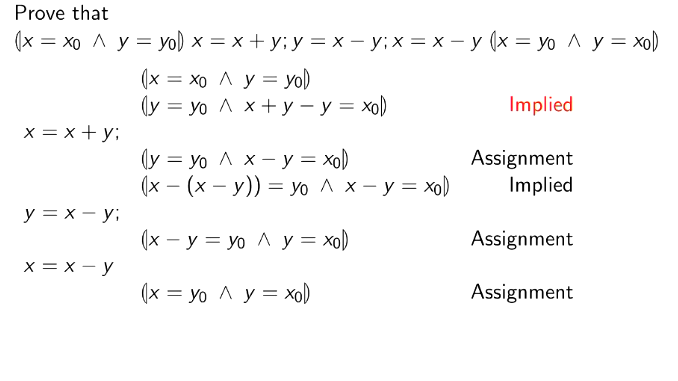
\includegraphics[width=0.8\textwidth]{three.png}
        	\caption{Example}
        	\label{fig:three-png}
        \end{figure}
\end{tcolorbox}
\begin{tcolorbox}[colback=black!3!white,colframe=black!60!white,title=\begin{defn}Conditional Rule \label{Conditional Rule}\end{defn}]
An if statement takes one of two branches, depending on whether the condition is true or false
\begin{align}
\frac{\llparenthesis Pre \land B \rrparenthesis C_1 \llparenthesis Post \rrparenthesis \;\; \; \; \; \; \; \; \; \llparenthesis Pre \land \neg B \rrparenthesis C_2 \llparenthesis Post \rrparenthesis}{\llparenthesis Pre \rrparenthesis \text{ if } B \{C_1\} \text{ else } \{ C_2 \} \llparenthesis Post \rrparenthesis}
\end{align}
\end{tcolorbox}
\begin{tcolorbox}[colback=black!3!white,colframe=black!60!white,title=\begin{exmp}Example \label{Example}\end{exmp}]
        \begin{figure}[H]
        	\centering
        	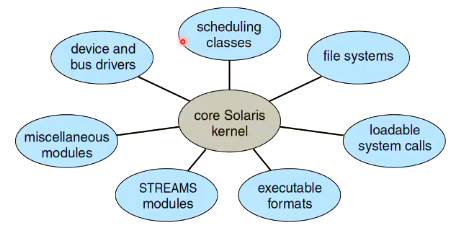
\includegraphics[width=0.8\textwidth]{four.png}
        	\caption{Example of Conditional Rule}
        	\label{fig:four-png}
        \end{figure}
                \begin{align}
                
                \end{align}
\end{tcolorbox}
\begin{tcolorbox}[colback=black!3!white,colframe=black!60!white,title=\begin{defn}Loop Rule \label{Loop Rule}\end{defn}]
A while statement is iterated as long as the condition is satisfied
\begin{align}
\frac{\llparenthesis B \land L \rrparenthesis C \llparenthesis L \rrparenthesis}{\llparenthesis L \rrparenthesis \text{ while } B \{ C \} \llparenthesis \neg B \land L \rrparenthesis}
\end{align}
L is called the loop invariant, it holds before and after each iteration. Finding a good loop variant is the key.
\end{tcolorbox}
\end{document}
